undefined
\documentclass[12pt,a4paper]{article}

% ------------------------- Packages -------------------------
\usepackage[margin=1in]{geometry}
\usepackage{graphicx}
\usepackage{float}
\usepackage{booktabs}
\usepackage{tabularx}
\usepackage{array}
\usepackage{longtable}
\usepackage{enumitem}
\usepackage{xcolor}
\usepackage{hyperref}
\usepackage{listings}
\usepackage{textcomp}
\usepackage{caption}
\usepackage{subcaption}
\usepackage{fancyhdr}
\usepackage{titlesec}
\usepackage{tikz}
\usetikzlibrary{arrows.meta,positioning,shapes.geometric,fit}
\usepackage{microtype}
\usepackage{setspace}
\usepackage{parskip}
\usepackage{lastpage}

% ------------------------- Colors -------------------------
\definecolor{navy}{HTML}{17324D}
\definecolor{blueaccent}{HTML}{2F6B9A}
\definecolor{lightblue}{HTML}{EAF2F8}
\definecolor{lightgray}{HTML}{F4F6F7}
\definecolor{darkgray}{HTML}{4D5656}
\definecolor{codegreen}{HTML}{2E7D32}
\definecolor{codepurple}{HTML}{6A1B9A}

% ------------------------- Hyperlinks -------------------------
\hypersetup{
    colorlinks=true,
    linkcolor=navy,
    urlcolor=blueaccent,
    citecolor=navy,
    pdftitle={Lab 4 - Weather Stations Monitoring Technical Report},
    pdfauthor={Ahmed Walaaeldin, Mazen Adel, Marwan Ahmed, Ahmed Ibrahim}
}

% ------------------------- Headings -------------------------
\titleformat{\section}
  {\Large\bfseries\color{navy}}
  {\thesection}{0.7em}{}
\titleformat{\subsection}
  {\large\bfseries\color{blueaccent}}
  {\thesubsection}{0.6em}{}
\titleformat{\subsubsection}
  {\normalsize\bfseries\color{darkgray}}
  {\thesubsubsection}{0.5em}{}

% ------------------------- Header / Footer -------------------------
\pagestyle{fancy}
\setlength{\headheight}{14pt}
\fancyhf{}
\fancyhead[L]{\small Net Centric Computing - Lab 4}
\fancyhead[R]{\small Weather Stations Monitoring}
\fancyfoot[C]{\small Page \thepage\ of \pageref{LastPage}}
\renewcommand{\headrulewidth}{0.4pt}
\renewcommand{\footrulewidth}{0.2pt}

% ------------------------- Listings -------------------------
\lstdefinestyle{code}{
    backgroundcolor=\color{lightgray},
    basicstyle=\ttfamily\small,
    breaklines=true,
    frame=single,
    rulecolor=\color{gray!35},
    numbers=left,
    numberstyle=\tiny\color{gray},
    keywordstyle=\color{blueaccent}\bfseries,
    commentstyle=\color{codegreen},
    stringstyle=\color{codepurple},
    showstringspaces=false,
    tabsize=2,
    columns=fullflexible,
    upquote=true
}
\lstset{style=code}

% ------------------------- Figure helper -------------------------
\newcommand{\reportfigure}[3]{%
\begin{figure}[H]
    \centering
    \IfFileExists{#1}{%
        \includegraphics[width=#2\textwidth,height=0.68\textheight,keepaspectratio]{#1}%
    }{%
        \fbox{\parbox[c][3.5cm][c]{0.86\textwidth}{%
            \centering\textbf{Screenshot required}\\[0.5em]\texttt{#1}%
        }}%
    }
    \caption{#3}
\end{figure}
}

% ------------------------- Document metadata -------------------------
\newcommand{\coursename}{Net Centric Computing}
\newcommand{\labtitle}{Lab 4 - Weather Stations Monitoring}
\newcommand{\academicyear}{Fall 2025--2026}
\newcommand{\faculty}{Faculty of Engineering - Alexandria University}
\newcommand{\department}{Computer and Communications Engineering}
\newcommand{\submissiondate}{\today}

\begin{document}

% ================================================================
% Title Page
% ================================================================
\hypersetup{pageanchor=false}
\begin{titlepage}
    \centering
    \vspace*{1.2cm}
    {\Large\bfseries \faculty\par}
    \vspace{0.25cm}
    {\large \department\par}
    \vspace{1.4cm}

    {\Huge\bfseries\color{navy} \labtitle\par}
    \vspace{0.45cm}
    {\Large\color{blueaccent} Technical Report\par}
    \vspace{1.0cm}

    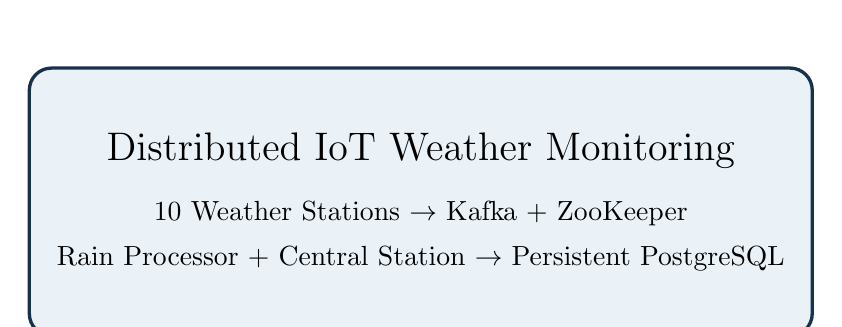
\begin{tikzpicture}
        \node[draw=navy, very thick, rounded corners=8pt, fill=lightblue,
              minimum width=0.82\textwidth, minimum height=3.4cm, align=center] {
            \Large Distributed IoT Weather Monitoring\\[0.35cm]
            \normalsize 10 Weather Stations $\rightarrow$ Kafka + ZooKeeper\\[0.15cm]
            Rain Processor + Central Station $\rightarrow$ Persistent PostgreSQL
        };
    \end{tikzpicture}

    \vfill
    \begin{tabular}{>{\bfseries}l l}
        Course: & \coursename \\
        Academic Year: & \academicyear \\
        Date: & \submissiondate \\
    \end{tabular}

    \vspace{0.8cm}
    {\large\bfseries Team Members\par}
    \vspace{0.3cm}
    \begin{tabular}{l r}
        \toprule
        \textbf{Name} & \textbf{ID} \\
        \midrule
        Ahmed Walaaeldin & 8625 \\
        Mazen Adel & 8634 \\
        Marwan Ahmed & 8824 \\
        Ahmed Ibrahim & 8672 \\
        \bottomrule
    \end{tabular}
    \vfill
\end{titlepage}
\hypersetup{pageanchor=true}

\tableofcontents
\newpage
\listoffigures
\newpage

% ================================================================
\section{Introduction}
% ================================================================
The objective of this lab is to implement a distributed weather monitoring system that models an Internet of Things (IoT) stream-processing pipeline. Multiple weather stations generate sensor readings, Apache Kafka provides asynchronous transport, a Kafka Streams processor detects rain conditions, and a central station stores historical data in a relational database.

Ten independent weather stations generate one sample per second. Each sample contains a station identifier, a per-station sequence number, battery status, Unix timestamp, humidity, temperature, and wind speed. Approximately 10\% of generated samples are intentionally dropped. Battery status is sampled using probabilities of 30\% low, 40\% medium, and 30\% high.

Weather readings are published to the \texttt{weather-readings} Kafka topic. A Kafka Streams processor identifies humidity values greater than 70\% and publishes corresponding messages to \texttt{rain-alerts}. The central station consumes both topics and persists the resulting records in PostgreSQL using batched database writes.

The complete system runs on Docker Desktop Kubernetes for macOS. The deployment includes a ZooKeeper-backed Kafka broker, ten weather station pods, a rain processor, a central station, and a PostgreSQL database backed by a 5~GiB PersistentVolume and PersistentVolumeClaim. Database persistence was verified by replacing the PostgreSQL pod and confirming that all previously stored readings and rain alerts remained available.

% ================================================================
\section{System Architecture}
% ================================================================
\subsection{High-Level Design}

\begin{figure}[H]
\centering
\resizebox{0.98\textwidth}{!}{%
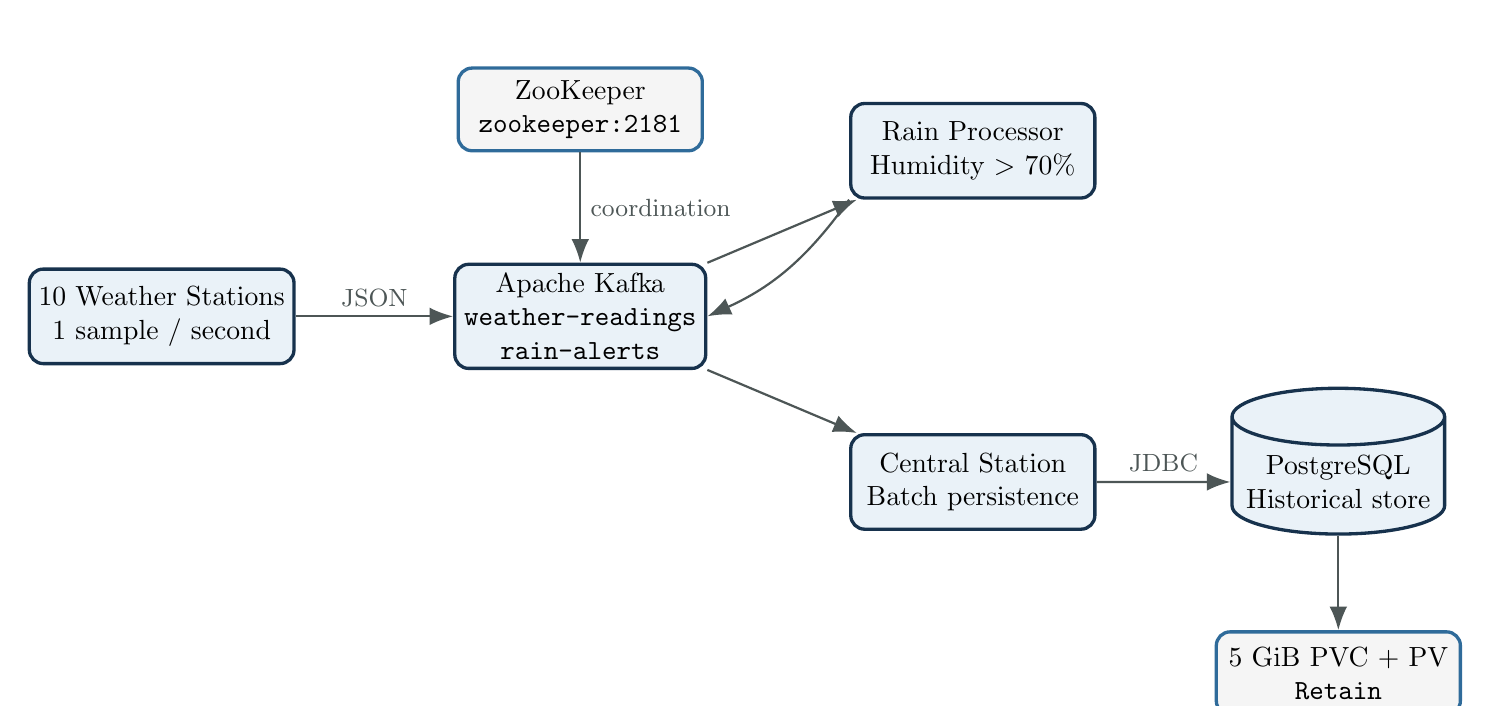
\begin{tikzpicture}[
    node distance=1.5cm and 1.8cm,
    box/.style={draw=navy, very thick, rounded corners=5pt,
                fill=lightblue, align=center, minimum height=1.2cm,
                minimum width=3.1cm},
    store/.style={draw=blueaccent, very thick, rounded corners=5pt,
                  fill=gray!8, align=center, minimum height=1.05cm,
                  minimum width=3.1cm},
    db/.style={draw=navy, very thick, cylinder, shape border rotate=90,
               aspect=0.28, fill=lightblue, minimum height=1.4cm,
               minimum width=2.7cm, align=center},
    arrow/.style={-{Latex[length=3mm]}, thick, color=darkgray}
]
    \node[box] (stations) {10 Weather Stations\\1 sample / second};
    \node[box, right=2.0cm of stations] (kafka)
        {Apache Kafka\\\texttt{weather-readings}\\\texttt{rain-alerts}};
    \node[store, above=1.4cm of kafka] (zookeeper)
        {ZooKeeper\\\texttt{zookeeper:2181}};
    \node[box, above right=0.8cm and 1.8cm of kafka] (rain)
        {Rain Processor\\Humidity $>$ 70\%};
    \node[box, below right=0.8cm and 1.8cm of kafka] (central)
        {Central Station\\Batch persistence};
    \node[db, right=1.7cm of central] (database)
        {PostgreSQL\\Historical store};
    \node[store, below=1.2cm of database] (storage)
        {5~GiB PVC + PV\\\texttt{Retain}};

    \draw[arrow] (stations) -- node[above, font=\small]{JSON} (kafka);
    \draw[arrow] (zookeeper) -- node[right, font=\small]{coordination} (kafka);
    \draw[arrow] (kafka) -- (rain);
    \draw[arrow] (rain.south west) to[bend left=15] (kafka.east);
    \draw[arrow] (kafka) -- (central);
    \draw[arrow] (central) -- node[above, font=\small]{JDBC} (database);
    \draw[arrow] (database) -- (storage);
\end{tikzpicture}%
}
\caption{Implemented Kubernetes architecture with ZooKeeper-backed Kafka and persistent PostgreSQL storage.}
\end{figure}

The architecture has three main stages:
\begin{enumerate}[label=\arabic*.]
    \item \textbf{Data acquisition:} ten weather station services generate simulated sensor readings and publish them to Kafka.
    \item \textbf{Data processing:} Kafka buffers the readings, while the rain processor produces alerts for humidity values above 70\%.
    \item \textbf{Data persistence and analysis:} the central station stores weather readings and rain alerts in PostgreSQL for historical analysis.
\end{enumerate}

Kafka separates producers from consumers and provides buffering, replay capability, per-key ordering, and independent processing of the two message streams. ZooKeeper coordinates the Kafka broker, while the PostgreSQL PersistentVolume separates database storage from the database pod lifecycle.

\subsection{Repository Organization}
The implementation is organized as a Maven multi-module project. The \texttt{common} module contains shared message classes and configuration helpers. Separate application modules implement the weather stations, rain processor, and central station. Kubernetes manifests, Dockerfiles, and SQL scripts are stored alongside the application source code.

\reportfigure{images/18-project-structure.png}{0.96}{Project repository structure showing application modules, Dockerfiles, SQL scripts, and Kubernetes manifests.}

\begin{table}[H]
\centering
\caption{Main repository components.}
\begin{tabularx}{\textwidth}{>{\ttfamily}l X}
\toprule
\textbf{Path} & \textbf{Purpose} \\
\midrule
common/ & Shared JSON models, Kafka topic names, and environment-based configuration helpers. \\
weather-station/ & Parts A and B: reading generation and Kafka production. \\
rain-processor/ & Part C: stateful Kafka Streams rain detection. \\
central-station/ & Part D: Kafka consumers, JDBC batching, and database initialization. \\
sql/ & Part E: relational schema and historical analysis queries. \\
k8s/ & Part F: ZooKeeper, Kafka, PostgreSQL, persistent storage, application manifests, and deployment script. \\
report/ & LaTeX report source, generated PDF, and supporting screenshots. \\
\bottomrule
\end{tabularx}
\end{table}

% ================================================================
\section{Weather Station Mock - Part A}
% ================================================================
\subsection{Reading Generation}
Each weather station generates one \texttt{WeatherMessage} every second. Its identity is supplied through the \texttt{STATION\_ID} environment variable or derived from its Kubernetes StatefulSet pod ordinal. Pod names \texttt{weather-station-0} through \texttt{weather-station-9} therefore correspond to logical station IDs 1 through 10.

The generated weather message has the following structure:

\begin{lstlisting}[language={},caption={Weather status JSON schema.}]
{
  "station_id": 1,
  "s_no": 1,
  "battery_status": "low",
  "status_timestamp": 1681521224,
  "weather": {
    "humidity": 35,
    "temperature": 100,
    "wind_speed": 13
  }
}
\end{lstlisting}

The sequence number increases for every generated sample before the message-drop decision. Consequently, intentionally dropped samples leave observable gaps in the stored sequence numbers.

\subsection{Battery Status Distribution}
A uniformly distributed random value $p \in [0,1)$ determines the battery state:

\begin{itemize}
    \item \texttt{low} when $p < 0.30$;
    \item \texttt{medium} when $0.30 \leq p < 0.70$;
    \item \texttt{high} when $p \geq 0.70$.
\end{itemize}

These thresholds produce the required theoretical distribution of 30\% low, 40\% medium, and 30\% high.

\subsection{Simulated Weather and Message Drops}
Humidity is generated between 0 and 100\%, temperature between 20 and 120 degrees Fahrenheit, and wind speed between 0 and 50~km/h. A second independent random draw drops approximately 10\% of generated samples. Dropped sequence numbers are not reused.

\reportfigure{images/01-weather-station-logs.png}{0.95}{Weather station logs showing generated readings and intentionally dropped messages.}

% ================================================================
\section{Kafka Integration - Part B}
% ================================================================
\subsection{Producer Configuration}
The weather station uses the Java Kafka Producer API to publish serialized JSON messages to the \texttt{weather-readings} topic. The principal producer settings are summarized below.

\begin{table}[H]
\centering
\caption{Weather station Kafka producer configuration.}
\begin{tabularx}{\textwidth}{l l X}
\toprule
\textbf{Property} & \textbf{Value} & \textbf{Reason} \\
\midrule
Bootstrap servers & Environment configured & Supports the deployed Kubernetes Kafka endpoint. \\
Key serializer & StringSerializer & Uses the station ID as the message key. \\
Value serializer & StringSerializer & Serializes weather messages as JSON strings. \\
\texttt{acks} & \texttt{all} & Requires acknowledgement from the available broker replicas. \\
Idempotence & enabled & Prevents duplicate producer writes caused by retries. \\
Retries & 3 & Handles transient Kafka communication failures. \\
\texttt{linger.ms} & 20~ms & Allows short producer-side batching. \\
Compression & gzip & Reduces the message payload transmitted over the network. \\
\bottomrule
\end{tabularx}
\end{table}

\subsection{Partitioning and Ordering}
The Kafka message key is the station ID. Readings from an individual station are therefore routed consistently to the same partition, preserving their relative order. The deployment creates ten partitions for both \texttt{weather-readings} and \texttt{rain-alerts}. Distinct station IDs can still map to the same partition because partition assignment is based on hashing rather than a dedicated partition per station.

\reportfigure{images/04-kafka-weather-readings.png}{0.98}{Weather message consumed directly from the Kafka weather-readings topic.}

\reportfigure{images/10-kafka-topics-list.png}{0.94}{Kafka topics for weather readings and rain alerts, each configured with ten partitions.}

% ================================================================
\section{Rain Detection - Part C}
% ================================================================
\subsection{Kafka Streams Processor API}
Rain detection uses the Kafka Streams Processor API. The processing topology is:

\begin{center}
\texttt{weather-readings} $\rightarrow$ \texttt{RainProcessor}
$\rightarrow$ \texttt{rain-alerts}
\end{center}

Each incoming record is deserialized into a \texttt{WeatherMessage}. Missing or malformed weather records are skipped. A rain alert is generated only when humidity is strictly greater than 70\%; a value of exactly 70\% does not trigger an alert. For qualifying records, the processor updates a per-station counter in its state store and forwards a \texttt{RainAlert}.

The alert includes the station ID, sequence number, timestamp, humidity, accumulated alert count, and the message \texttt{It is raining}.

\subsection{Processor API Versus DSL}
The project also includes an alternative Kafka Streams DSL implementation. The DSL expresses the transformation through stream operations such as \texttt{mapValues}, \texttt{filter}, and \texttt{to}. The Processor API implementation is used for the primary deployment because it provides direct access to the per-station state store and explicit control over record forwarding.

\reportfigure{images/02-rain-processor-logs.png}{0.95}{Rain processor detecting humidity values greater than 70\%.}

\reportfigure{images/05-kafka-rain-alerts.png}{0.98}{Rain-alert message consumed from the Kafka rain-alerts topic.}

% ================================================================
\section{Central Station - Part D}
% ================================================================
\subsection{Concurrent Consumers}
The central station initializes the PostgreSQL schema and runs two Kafka consumers in separate threads:

\begin{itemize}
    \item a weather-reading consumer subscribed to \texttt{weather-readings};
    \item a rain-alert consumer subscribed to \texttt{rain-alerts}.
\end{itemize}

The consumers use separate JDBC connections and manual Kafka offset commits.

\subsection{Batch Persistence}
The weather-reading consumer buffers messages and flushes them to PostgreSQL when either the configured threshold of 5,000 records is reached or the 10-second flush interval expires while records are pending.

At the normal rate of approximately ten generated samples per second across all stations, timed batches are usually much smaller than 5,000 records. The batch writer uses a prepared statement and JDBC \texttt{executeBatch()} to persist multiple records in a single transaction.

\subsection{Delivery Semantics and Idempotency}
The persistence sequence is:

\begin{enumerate}[label=\arabic*.]
    \item insert the weather-reading batch into PostgreSQL;
    \item commit the PostgreSQL transaction;
    \item commit the corresponding Kafka offsets.
\end{enumerate}

This ordering provides at-least-once processing. If a failure occurs after the database transaction commits but before the Kafka offsets commit, the same records can be consumed again. The uniqueness constraint \texttt{UNIQUE(station\_id, sequence\_number)} and an \texttt{ON CONFLICT DO NOTHING} insert prevent duplicated historical readings.

\subsection{Database Schema}
The main table stores all weather readings. A second table archives rain alerts, and the \texttt{latest\_station\_status} view retrieves the newest reading for each station.

\begin{lstlisting}[language=SQL,caption={Core weather readings schema.}]
CREATE TABLE IF NOT EXISTS weather_readings (
    id              BIGSERIAL PRIMARY KEY,
    station_id      BIGINT      NOT NULL,
    sequence_number BIGINT      NOT NULL,
    battery_status  VARCHAR(10) NOT NULL,
    timestamp       BIGINT      NOT NULL,
    humidity        INT,
    temperature     INT,
    wind_speed      INT,
    ingested_at     TIMESTAMPTZ NOT NULL DEFAULT now(),
    CONSTRAINT uq_station_sequence
        UNIQUE (station_id, sequence_number)
);
\end{lstlisting}

\reportfigure{images/03-central-station-logs.png}{0.96}{Central station consuming Kafka messages and persisting weather readings and rain alerts.}

% ================================================================
\section{Historical Weather Analysis - Part E}
% ================================================================
SQL queries validate the battery-status distribution, estimate dropped messages, retrieve the latest weather status, and compare rain alerts with qualifying weather readings.

\subsection{Battery Status Distribution Per Station}
The following query groups records by station and calculates the percentage of low, medium, and high battery states.

\begin{lstlisting}[language=SQL,caption={Battery distribution query.}]
SELECT
    station_id,
    COUNT(*) AS total_readings,
    ROUND(
        100.0 * COUNT(*) FILTER (
            WHERE battery_status = 'low'
        ) / COUNT(*), 2
    ) AS low_pct,
    ROUND(
        100.0 * COUNT(*) FILTER (
            WHERE battery_status = 'medium'
        ) / COUNT(*), 2
    ) AS medium_pct,
    ROUND(
        100.0 * COUNT(*) FILTER (
            WHERE battery_status = 'high'
        ) / COUNT(*), 2
    ) AS high_pct
FROM weather_readings
GROUP BY station_id
ORDER BY station_id;
\end{lstlisting}

\reportfigure{images/06-battery-distribution.png}{0.98}{Measured battery-status distribution for all ten weather stations.}

Small deviations from the configured 30\% / 40\% / 30\% probabilities are expected because the readings are generated randomly. Larger sample sizes reduce the relative variation.

\subsection{Dropped Messages Per Station}
Because the sequence number increases before the drop decision, missing sequence numbers can be estimated by comparing the largest observed sequence number with the number of stored readings.

\begin{lstlisting}[language=SQL,caption={Dropped-message estimation query.}]
SELECT
    station_id,
    MAX(sequence_number) AS expected_messages,
    COUNT(*) AS received_messages,
    MAX(sequence_number) - COUNT(*) AS dropped_messages,
    ROUND(
        100.0 * (MAX(sequence_number) - COUNT(*))
        / NULLIF(MAX(sequence_number), 0),
        2
    ) AS drop_rate_pct
FROM weather_readings
GROUP BY station_id
ORDER BY station_id;
\end{lstlisting}

\reportfigure{images/07-dropped-messages.png}{0.98}{Estimated dropped-message count and drop percentage for each weather station.}

The expected drop percentage is approximately 10\%. This calculation assumes the stored history includes the beginning of each station's sequence.

\subsection{Latest Weather Status Per Station}
The latest status for each station can be retrieved directly from PostgreSQL by selecting the largest observed sequence number.

\begin{lstlisting}[language=SQL,caption={Latest weather status for each station.}]
SELECT DISTINCT ON (station_id)
    station_id,
    sequence_number,
    battery_status,
    humidity,
    temperature,
    wind_speed
FROM weather_readings
ORDER BY station_id, sequence_number DESC;
\end{lstlisting}

\reportfigure{images/08-latest-weather-status.png}{0.98}{Latest weather reading retrieved directly from PostgreSQL for each station.}

\subsection{Rain Alert Cross-Check}
Weather readings are inserted in timed batches, while rain alerts can be persisted sooner. Consequently, a simple comparison of live aggregate counts can temporarily differ even when processing is correct. A more useful cross-check joins older high-humidity readings to rain alerts by station ID and sequence number.

\begin{lstlisting}[language=SQL,caption={Per-station rain-alert validation.}]
WITH eligible_readings AS (
    SELECT station_id, sequence_number
    FROM weather_readings
    WHERE humidity > 70
      AND ingested_at < NOW() - INTERVAL '30 seconds'
)
SELECT
    r.station_id,
    COUNT(*) AS qualifying_readings,
    COUNT(a.sequence_number) AS matching_alerts,
    COUNT(*) FILTER (
        WHERE a.sequence_number IS NULL
    ) AS missing_alerts
FROM eligible_readings r
LEFT JOIN rain_alerts a
    ON a.station_id = r.station_id
   AND a.sequence_number = r.sequence_number
GROUP BY r.station_id
ORDER BY r.station_id;
\end{lstlisting}

\reportfigure{images/09-rain-alerts-cross-check.png}{0.98}{Per-station cross-check between high-humidity readings and their corresponding rain alerts.}

% ================================================================
\section{Kubernetes Deployment - Part F}
% ================================================================
\subsection{Deployment Environment and Containerization}
The system runs on Docker Desktop Kubernetes for macOS in the \texttt{weather} namespace. The Weather Station, Rain Processor, and Central Station each use a multi-stage Dockerfile. Maven and Eclipse Temurin JDK~17 build the applications, while the runtime containers contain Eclipse Temurin JRE~17 and the application JAR.

\subsection{Kubernetes Resources}
The Kubernetes deployment defines independent resources for configuration, ZooKeeper, Kafka, PostgreSQL, persistent database storage, the weather stations, the rain processor, and the central station.

\begin{table}[H]
\centering
\caption{Kubernetes resource inventory.}
\begin{tabularx}{\textwidth}{l X}
\toprule
\textbf{Resource} & \textbf{Role} \\
\midrule
Namespace \texttt{weather} & Isolates the resources used by the lab deployment. \\
ConfigMap \texttt{weather-config} & Stores Kafka endpoints, topic names, emission timing, drop rate, batch size, and database URL. \\
Secret \texttt{db-credentials} & Supplies PostgreSQL credentials to the relevant containers. \\
ZooKeeper Deployment and Service & Coordinates Kafka through \texttt{zookeeper:2181}. \\
Kafka Deployment and Service & Exposes the broker to cluster clients at \texttt{kafka:9092}. \\
Kafka topic-initialization Job & Creates the two application topics with ten partitions. \\
PostgreSQL Deployment and Service & Provides the relational historical database. \\
PostgreSQL PV and PVC & Persist database files independently of the PostgreSQL pod. \\
Weather Station StatefulSet & Runs ten replicas with stable ordinal identities. \\
Rain Processor Deployment & Executes Kafka Streams rain detection. \\
Central Station Deployment & Consumes both topics and writes to PostgreSQL. \\
\bottomrule
\end{tabularx}
\end{table}

ZooKeeper and Kafka use \texttt{01-zookeeper.yaml} and \texttt{02-kafka.yaml}. The PostgreSQL storage resources use \texttt{02-postgres-storage.yaml}. The database Deployment and Service are configured in \texttt{02-postgres.yaml}.

\reportfigure{images/11-k8s-all-pods.png}{0.98}{Kubernetes pods for ZooKeeper, Kafka, PostgreSQL, ten weather stations, the rain processor, and the central station.}

\reportfigure{images/15-k8s-services-statefulset.png}{0.98}{Kubernetes Services, application Deployments, topic-initialization Job, and the ten-replica Weather Station StatefulSet.}

\subsection{Kafka and ZooKeeper Coordination}
Kafka runs from the Bitnami Legacy Kafka~3.6 image, and ZooKeeper uses the official ZooKeeper~3.9 image. The broker connects to \texttt{zookeeper:2181}, and KRaft mode is disabled. Successful broker registration under \texttt{/brokers/ids/1} confirms that ZooKeeper actively coordinates Kafka.

\begin{lstlisting}[language=bash,caption={ZooKeeper-backed Kafka verification.}]
kubectl -n weather exec deploy/kafka -- \
  printenv KAFKA_CFG_ZOOKEEPER_CONNECT

kubectl -n weather exec deploy/kafka -- \
  printenv KAFKA_ENABLE_KRAFT

kubectl -n weather logs deploy/kafka | \
  grep 'Registered broker'

kubectl -n weather exec deploy/zookeeper -- \
  zkCli.sh -server localhost:2181 ls /brokers/ids
\end{lstlisting}

\reportfigure{images/19-k8s-zookeeper-verification.png}{0.98}{Kafka ZooKeeper connection and successful registration of broker 1.}

\subsection{Weather Station StatefulSet}
The Weather Station StatefulSet provides stable pod names from \texttt{weather-station-0} through \texttt{weather-station-9}. The application maps the pod ordinal to logical station IDs 1 through 10, avoiding ten separate Deployment manifests. A headless Service supports the StatefulSet's network identities.

\subsection{PostgreSQL Persistent Storage}
PostgreSQL mounts the \texttt{weather-postgres-pvc} claim at \texttt{/var/lib/postgresql/data}. The claim is bound to the 5~GiB \texttt{weather-postgres-pv} PersistentVolume, which uses \texttt{ReadWriteOnce} access and a \texttt{Retain} reclaim policy.

The PersistentVolume is backed by a local \texttt{hostPath} on the Docker Desktop Kubernetes node. This preserves database files across PostgreSQL pod replacement on that node. It does not provide protection against deleting or resetting the complete Kubernetes cluster.

\begin{lstlisting}[language=bash,caption={PostgreSQL persistent-storage verification.}]
kubectl get pv weather-postgres-pv

kubectl -n weather get pvc weather-postgres-pvc

kubectl -n weather get deployment postgres \
  -o jsonpath='{.spec.template.spec.volumes[0].persistentVolumeClaim.claimName}'
\end{lstlisting}

\reportfigure{images/20-k8s-postgres-persistent-storage.png}{0.98}{Bound PostgreSQL PersistentVolume and PersistentVolumeClaim mounted by the PostgreSQL Deployment.}

\subsection{Database Persistence Verification}
Database persistence was tested by temporarily stopping the central station, recording the number of rows in both PostgreSQL tables, replacing the PostgreSQL pod, and repeating the same queries after the replacement pod became ready.

\begin{table}[H]
\centering
\caption{PostgreSQL row counts before and after pod replacement.}
\begin{tabular}{l r r}
\toprule
\textbf{Database table} & \textbf{Before restart} & \textbf{After restart} \\
\midrule
\texttt{weather\_readings} & 114,804 & 114,804 \\
\texttt{rain\_alerts} & 15,061 & 15,061 \\
\bottomrule
\end{tabular}
\end{table}

Both counts remained unchanged, demonstrating that the replacement PostgreSQL pod reused the existing PersistentVolumeClaim. After the central station was scaled back to one replica, the number of weather readings increased to 51,404, confirming that normal ingestion resumed.

\reportfigure{images/21-k8s-postgres-persistence-test.png}{0.98}{PostgreSQL pod-replacement test confirming that weather readings and rain alerts survived the restart.}

\subsection{Configuration and Secrets}
Application settings are supplied through the \texttt{weather-config} ConfigMap. The configured emission interval is 1,000~ms, the drop rate is 0.10, the batch threshold is 5,000 records, and the flush interval is 10,000~ms. Database credentials are injected from the \texttt{db-credentials} Kubernetes Secret rather than being hardcoded in application source files.

\reportfigure{images/16-k8s-configmap-secret.png}{0.98}{Kubernetes ConfigMap values and database Secret metadata without exposing credential values.}

\subsection{Runtime Evidence}
The following screenshots show the application operating inside Kubernetes: weather readings are generated, qualifying humidity values produce alerts, the central station persists batches, and the database can be queried from the cluster.

\reportfigure{images/14-k8s-weather-station-0.png}{0.96}{Weather station pod logs showing generated readings and simulated message drops.}

\reportfigure{images/13-k8s-rain-processor.png}{0.96}{Rain Processor running in Kubernetes and detecting humidity values greater than 70\%.}

\reportfigure{images/12-k8s-central-batch-inserts.png}{0.96}{Central Station logs showing JDBC batch persistence inside Kubernetes.}

\reportfigure{images/17-k8s-database-results.png}{0.98}{PostgreSQL query results obtained from the Kubernetes deployment.}

% ================================================================
\section{Challenges and Lessons Learned}
% ================================================================
The implementation and deployment demonstrated several practical distributed-system concerns:

\begin{itemize}
    \item \textbf{Kafka coordination must match the deployment requirement.} The original Kafka setup used KRaft mode. Replacing it with a ZooKeeper-compatible broker and verifying broker registration satisfied the required Kafka-plus-ZooKeeper architecture.

    \item \textbf{Container image availability affects reproducibility.} The original Bitnami image tags were unavailable. The replacement images are the official ZooKeeper~3.9 image and Bitnami Legacy Kafka~3.6.

    \item \textbf{Persistent storage requires explicit migration.} Existing PostgreSQL data was backed up, restored into a PVC-backed database, and verified before and after pod replacement.

    \item \textbf{Random simulation must remain measurable.} Incrementing \texttt{s\_no} before the drop decision makes missing samples observable through sequence-number gaps.

    \item \textbf{Partition keys preserve per-station ordering.} Using \texttt{station\_id} as the Kafka key keeps records from the same station in a consistent partition, although different stations can share a partition.

    \item \textbf{Database writes and offset commits must be coordinated.} Committing PostgreSQL before Kafka offsets, combined with a uniqueness constraint, supports idempotent recovery.

    \item \textbf{Batching balances throughput and latency.} A 5,000-record threshold and a 10-second flush interval reduce database I/O without indefinitely delaying low-volume traffic.

    \item \textbf{Kubernetes resources have distinct responsibilities.} StatefulSets provide stable station identities, Secrets protect credentials, and PersistentVolumes preserve database contents across pod replacement.
\end{itemize}

% ================================================================
\section{Conclusion}
% ================================================================
The project implements the required distributed weather monitoring system using ten simulated weather stations, Apache Kafka, ZooKeeper, a Kafka Streams rain processor, a central station, and PostgreSQL. Each station generates one sample per second, applies the required battery-status probabilities, and intentionally drops approximately 10\% of generated samples.

Weather readings are published to Kafka, and readings with humidity greater than 70\% generate alerts on a separate topic. The central station consumes both streams and persists their records in PostgreSQL using batched database writes. SQL analysis validates battery distributions, estimates dropped messages, retrieves the latest station status, and checks the relationship between qualifying readings and generated alerts.

The complete system is deployed on Docker Desktop Kubernetes. Kafka operates with an active ZooKeeper service, and PostgreSQL uses a 5~GiB PersistentVolume and PersistentVolumeClaim. A controlled PostgreSQL pod-replacement test preserved all 114,804 weather readings and 15,061 rain alerts, demonstrating that database contents remain available across the lifecycle of the PostgreSQL pod.

\end{document}
undefined